\documentclass[11pt,a4paper]{article}
\usepackage[T1]{fontenc}
\usepackage[margin=2.3cm]{geometry}
\usepackage{amsmath,amssymb}
\usepackage{graphicx}
\usepackage[dvipsnames]{xcolor}
\usepackage{enumitem}
\usepackage[colorlinks=true,linkcolor=blue,urlcolor=blue]{hyperref}
\setlength{\parskip}{0.6em}
\setlength{\parindent}{0pt}
\begin{document}

\begin{center}{\LARGE\bfseries openbuildingsway}\\[0.4em]{\large Predict how a building sways in an earthquake, floor by floor.}\\[0.2em]\small PAN IIT OSS explainer \textbullet{} diploma / undergraduate to advanced undergraduate (levels 5-6)\end{center}

\section*{Why this exists}
A building is a stack of floors held up by springy columns, and when the ground shakes it sways in several patterns at once. This explainer follows the mathematics from one mass on a spring to a ten-storey frame, using only simple matrices and a few lines of code, so you can build it yourself.

\section*{The end goal}
Predict building sway in an earthquake with multi-DOF vibration. The end goal is predicting building sway in an earthquake with multi-degree-of-freedom vibration: periods, mode shapes, drift and base shear for a shear building, validated against exact results. It is an educational model, never a method for seismic design, which needs qualified engineers, building codes and far richer models.

\section*{How the three sessions build up}
\begin{enumerate}[nosep]
\item \textbf{Session 1: A building is a mass on a spring} (Level 1, conceptual interactive model, 60 min).
\item \textbf{Session 2: One storey, one rhythm: resonance and stiffness design} (Level 2, mathematical engineering model, 75 min).
\item \textbf{Session 3: Many floors, many modes: a ten-storey frame in an earthquake} (Level 3, simulation and validation, 90 min).
\end{enumerate}

\section{Session 1: A building is a mass on a spring}

\subsection*{A. Real-world problem}
After an earthquake some buildings are badly shaken while the one next door hardly moves. Part of the answer is rhythm. Every building has its own slow, regular sway, and the ground has a favourite rhythm too. If the two match, each shove adds to the last, like pushing a child on a swing at just the right moment. What decides a building's rhythm, and how bad is the match? (This repo is for learning. It is a simplified model and must never be used to design or judge a real building.)

\subsection*{B. Concept and theory}
Picture the whole building as one lump of mass m on one spring of stiffness k, where k is the sideways force needed per metre of sway. Pull it sideways and let go: it swings back and forth. The angular frequency w = sqrt(k / m) tells how fast the cycle goes in radians per second, and the period T = 2 pi / w is the time for one full back-and-forth sway. Heavier means slower, stiffer means faster. For typical frame buildings engineers often use the rough empirical rule of thumb T about 0.1 N seconds for N storeys; it is only a guide. When the ground is shaken back and forth with period Tg, the gain says how much the sway is amplified compared with a very slow push. With r = T / Tg and a damping ratio zeta (typically 0.05, meaning the sway dies away by a few percent each cycle), the gain is 1 / sqrt((1 - r\textasciicircum{}2)\textasciicircum{}2 + (2 zeta r)\textasciicircum{}2). Session 2 derives it.

\begin{itemize}[nosep]
\item m: mass of the building lump (kg)
\item k: sideways stiffness of the columns (N/m)
\item w: angular frequency of the sway (rad/s)
\item T: period of the sway (s)
\item Tg: period of the ground shaking (s)
\item r: ratio T / Tg (no unit)
\item zeta: damping ratio (no unit)
\item gain: sway divided by the sway for a very slow push (no unit)
\end{itemize}

\begin{equation*}
\omega=\sqrt{\frac{k}{m}},\qquad T=\frac{2\pi}{\omega}
\end{equation*}

\begin{equation*}
x(t)=x_0\cos(\omega t)\quad\text{(free sway released from rest at }x_0\text{)}
\end{equation*}

\begin{equation*}
T\approx 0.1\,N\ \text{s}\quad\text{(rough empirical rule of thumb for typical frame buildings)}
\end{equation*}

\begin{equation*}
\text{gain}=\frac{1}{\sqrt{(1-r^2)^2+(2\zeta r)^2}},\qquad r=\frac{T}{T_g}
\end{equation*}

\begin{center}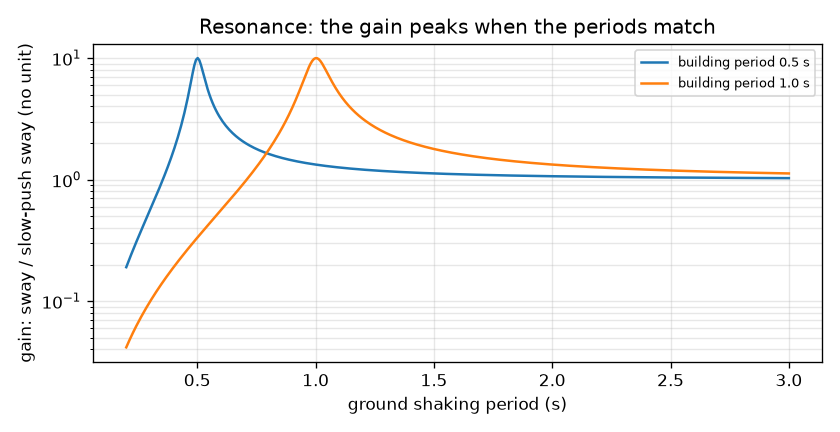
\includegraphics[width=0.85\linewidth]{figures/s01_gain_vs_ground_period.png}\\\small Gain against ground period for buildings of 0.5 s and 1 s: the peak of 10 sits where the periods match.\end{center}

\subsection*{E. Worked example}
A building lump has m = 200 000 kg and k = 20 000 000 N/m. Find w and T. What happens to T if the mass doubles, and if the stiffness is multiplied by four? At resonance with 5 percent damping, how much is the sway amplified?
\begin{enumerate}[nosep]
\item w = sqrt(k / m) = sqrt(20 000 000 / 200 000) = sqrt(100) = 10 rad/s.
\item T = 2 pi / w = 6.283 / 10 = 0.6283 s.
\item Double the mass: T grows by a factor sqrt(2), so T = 0.6283 * 1.4142 = 0.8886 s.
\item Four times the stiffness: T shrinks by a factor sqrt(4) = 2, so T = 0.3142 s.
\item At resonance r = 1, so the gain is 1 / sqrt(0 + (2 * 0.05 * 1)\textasciicircum{}2) = 1 / 0.1 = 10.
\end{enumerate}
\textbf{Answer.} w = 10 rad/s and T = 0.6283 s; doubling the mass gives 0.8886 s, quadrupling the stiffness gives 0.3142 s; at resonance the gain is 10.

\subsection*{F. Questions}
\begin{enumerate}[nosep]
\item \textbf{Conceptual.} Why does a heavier building sway more slowly while a stiffer building sways faster? Why can a matching ground rhythm be dangerous even when the push itself is small?
\item \textbf{Numerical.} A building lump has m = 500 000 kg and k = 20 000 000 N/m. Find w and T and say whether it is close to the 1 s ground period.
\item \textbf{Graph and simulation interpretation.} On the gain graph a 1 s building is shaken by a ground whose period is 2 s, and then by one with period 0.5 s. Read the gain in each case and say what each tells an engineer.
\item \textbf{Design and optimisation challenge.} A building has m = 200 000 kg and the ground period is 1 s. Choose a stiffness k that makes its period 0.5 s (a stiff design) or 1.5 s (a flexible design). What does each give for the gain, and what is the downside of each?
\end{enumerate}

\section{Session 2: One storey, one rhythm: resonance and stiffness design}

\subsection*{A. Real-world problem}
Soft soils in many cities shake mostly with a period near 1 s. A one-storey building has a roof mass of 200 tonnes on columns whose stiffness makes its period exactly 1 s. How large does it sway if the ground shakes with an acceleration of 2 m/s\textasciicircum{}2? And how stiff must the columns be to move the building safely away from that rhythm? (Educational model only, never for real design.)

\subsection*{B. Concept and theory}
Let u be the roof displacement relative to the ground. Newton's law for the roof mass m, with a spring k, a damper c and the ground acceleration a\_g(t), gives m u'' + c u' + k u = -m a\_g. Dividing by m and writing w = sqrt(k / m) and zeta = c / (2 m w) gives u'' + 2 zeta w u' + w\textasciicircum{}2 u = -a\_g(t). For ground acceleration a0 sin(W t) the sway settles, after a short transient, into a steady wave with amplitude u\_max = (a0 / w\textasciicircum{}2) D(r), where r = W / w is the frequency ratio and D(r) = 1 / sqrt((1 - r\textasciicircum{}2)\textasciicircum{}2 + (2 zeta r)\textasciicircum{}2) is the amplification factor. Since W = 2 pi / Tg and w = 2 pi / T, the ratio is also r = T / Tg. The factor a0 / w\textasciicircum{}2 is the sway if the acceleration were applied as a constant push. D is largest at r = sqrt(1 - 2 zeta\textasciicircum{}2) (close to 1) and its maximum is about 1 / (2 zeta); for the typical zeta = 0.05 that is about 10. The rule of thumb T about 0.1 N seconds is a rough empirical guide for N-storey frame buildings.

\begin{itemize}[nosep]
\item m: roof mass (kg)
\item k: storey stiffness (N/m)
\item c: damping coefficient (N s/m)
\item zeta: damping ratio c / (2 m w) (no unit)
\item w: natural angular frequency sqrt(k / m) (rad/s)
\item T, Tg: natural period of the building, period of the ground shaking (s)
\item a0: amplitude of the ground acceleration (m/s\textasciicircum{}2)
\item r: frequency ratio W / w = T / Tg (no unit)
\item D: amplification factor (no unit)
\item u\_max: steady sway amplitude relative to the ground (m)
\end{itemize}

\begin{equation*}
m\ddot u+c\dot u+ku=-m\,a_g(t)\;\Longrightarrow\;\ddot u+2\zeta\omega\dot u+\omega^2u=-a_g(t)
\end{equation*}

\begin{equation*}
\omega=\sqrt{k/m},\quad T=\frac{2\pi}{\omega},\quad \zeta=\frac{c}{2m\omega},\quad r=\frac{\Omega}{\omega}=\frac{T}{T_g}
\end{equation*}

\begin{equation*}
u_{\max}=\frac{a_0}{\omega^2}\,D(r),\qquad D(r)=\frac{1}{\sqrt{(1-r^2)^2+(2\zeta r)^2}}
\end{equation*}

\begin{equation*}
D_{\max}=\frac{1}{2\zeta\sqrt{1-\zeta^2}}\approx\frac{1}{2\zeta}\quad\text{at } r=\sqrt{1-2\zeta^2}
\end{equation*}

\begin{equation*}
k=m\left(\frac{2\pi}{T}\right)^2
\end{equation*}

\begin{center}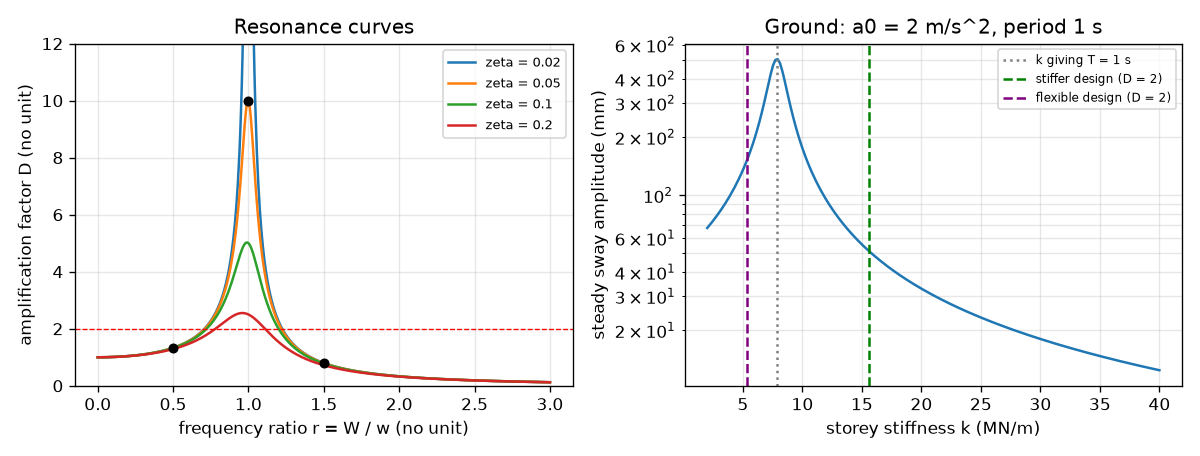
\includegraphics[width=0.85\linewidth]{figures/s02_resonance_and_design.png}\\\small Left: amplification factor against frequency ratio for four dampings, with numerical dots. Right: steady sway against storey stiffness, with the stiff and flexible design points.\end{center}

\subsection*{E. Worked example}
A roof mass m = 200 000 kg sits on columns of period T = 1 s. (a) Find k. (b) For a ground acceleration amplitude of 2 m/s\textasciicircum{}2 and a period of 1 s with zeta = 0.05, find the steady sway. (c) How stiff must the columns be so that D is at most 2 on the stiff side?
\begin{enumerate}[nosep]
\item k = m (2 pi / T)\textasciicircum{}2 = 200 000 * (6.2832)\textasciicircum{}2 = 200 000 * 39.478 = 7.896e6 N/m, and w = 2 pi / 1 = 6.283 rad/s.
\item At T = Tg = 1 s, r = 1, so D = 1 / (2 zeta) = 10.
\item a0 / w\textasciicircum{}2 = 2 / 39.478 = 0.05066 m, so u\_max = 0.05066 * 10 = 0.5066 m: more than half a metre.
\item For (c) solve D(r) = 2 with r below 1: (1 - r\textasciicircum{}2)\textasciicircum{}2 + (0.1 r)\textasciicircum{}2 = 0.25. This gives r = 0.7107 (r\textasciicircum{}2 = 0.505, 1 - r\textasciicircum{}2 = 0.495, and 0.495\textasciicircum{}2 + 0.0051 = 0.250).
\item The building period must be T = r Tg = 0.7107 s, so k = m (2 pi / 0.7107)\textasciicircum{}2 = 1.563e7 N/m, about 1.98 times the original stiffness.
\end{enumerate}
\textbf{Answer.} k = 7.896e6 N/m gives resonance with a sway of 0.5066 m for D = 10. Making the columns 1.98 times stiffer (k = 1.563e7 N/m, T = 0.7107 s) brings D down to 2. A much more flexible building also works: D = 2 at r = 1.2186, T = 1.2186 s and k = 5.317e6 N/m (0.673 times the original).

\subsection*{F. Questions}
\begin{enumerate}[nosep]
\item \textbf{Conceptual.} Why does the amplification factor go above 1 near r = 1 but fall below 1 for large r? What does damping change?
\item \textbf{Numerical.} A storey has m = 100 000 kg and k = 4e6 N/m, damping 5 percent. The ground has period 1 s and acceleration amplitude 2 m/s\textasciicircum{}2. Find w, T, r, D and the steady sway amplitude.
\item \textbf{Graph and simulation interpretation.} On the resonance curves, read D at r = 1 for zeta = 0.02, 0.05, 0.1 and 0.2, and D at r = 1.5 for zeta = 0.05. What does each tell you?
\item \textbf{Design and optimisation challenge.} The ground period is 1.5 s (softer soil) and the roof mass is 200 000 kg. Find the stiffness and the building period for D = 2 on the stiff side and on the flexible side, with the sway amplitude for a0 = 2 m/s\textasciicircum{}2. Which design would you prefer and why?
\end{enumerate}

\section{Session 3: Many floors, many modes: a ten-storey frame in an earthquake}

\subsection*{A. Real-world problem}
A real building is not one lump: each floor is a mass, each storey of columns is a spring, and the stack can bend in many patterns at once. For a ten-storey frame with a first period near 1 s, how large is the sway at each floor in a synthetic earthquake record, which storey is bent most, how big is the force at the base, and what happens if one storey is much weaker than the rest? Can we trust the answer? (A simplified, linear, planar model for learning, never for seismic design.)

\subsection*{B. Concept and theory}
Number the floors 1 to N from the bottom; floor 0 is the fixed ground. Let u\_j be the sway of floor j relative to the ground, m\_j its mass, and k\_j the stiffness of storey j, between floors j - 1 and j. The equation of motion is M u'' + C u' + K u = -M r a\_g(t), where M is diagonal, K is tridiagonal (each floor feels only its two neighbours) and r is a vector of ones. Free vibration u = phi cos(w t) gives the generalised eigenproblem K phi = w\textasciicircum{}2 M phi. Because M is diagonal, put phi = M\textasciicircum{}(-1/2) v to get the ordinary symmetric problem (M\textasciicircum{}(-1/2) K M\textasciicircum{}(-1/2)) v = w\textasciicircum{}2 v, which np.linalg.eigh solves. The columns phi\_i are the mode shapes (scaled so phi\textasciicircum{}T M phi = 1) and w\_i the frequencies. For equal masses m and equal storey stiffness k, with a fixed base and a free top, the standard exact result is w\_i = 2 sqrt(k / m) sin((2i - 1) pi / (2(2N + 1))) with shape sin((2i - 1) j pi / (2N + 1)) at floor j; we verify it numerically. The ground motion couples to mode i through the participation factor Gamma\_i = phi\_i\textasciicircum{}T M r, and the effective modal mass Gamma\_i\textasciicircum{}2 measures how much of the total mass that mode moves; the effective masses of all modes add up to the total mass. Each mode obeys q'' + 2 zeta w q' + w\textasciicircum{}2 q = -Gamma a\_g(t) and u = sum of phi\_i q\_i (modal superposition). Alternatively the full equation is stepped directly by the Newmark-beta method with the average acceleration parameters beta = 1/4 and gamma = 1/2 (unconditionally stable, no numerical damping). The damping matrix C = M Phi diag(2 zeta w) Phi\textasciicircum{}T M gives the same zeta in every mode. Design quantities are the inter-storey drift u\_j - u\_(j-1) (drift ratio = drift / storey height), and the base shear = k\_1 u\_1, the force in the lowest storey.

\begin{itemize}[nosep]
\item N: number of storeys (no unit)
\item m: mass of one floor (kg)
\item k: stiffness of one storey (N/m)
\item M, K, C: mass, stiffness and damping matrices (kg, N/m, N s/m)
\item u: floor sway relative to the ground (vector) (m)
\item w\_i, phi\_i: frequency and mode shape of mode i (rad/s, shape)
\item Gamma\_i: participation factor of mode i (kg\textasciicircum{}(1/2))
\item a\_g(t): ground acceleration (synthetic record) (m/s\textasciicircum{}2)
\item zeta: damping ratio in every mode (0.05) (no unit)
\item V: base shear, k1 u1 (N)
\end{itemize}

\begin{equation*}
M\ddot{\mathbf u}+C\dot{\mathbf u}+K\mathbf u=-M\mathbf r\,a_g(t)
\end{equation*}

\begin{equation*}
K\boldsymbol\phi=\omega^2M\boldsymbol\phi\;\Longleftrightarrow\;(M^{-1/2}KM^{-1/2})\mathbf v=\omega^2\mathbf v,\quad \boldsymbol\phi=M^{-1/2}\mathbf v
\end{equation*}

\begin{equation*}
\omega_i=2\sqrt{\frac{k}{m}}\sin\frac{(2i-1)\pi}{2(2N+1)},\qquad \phi_{j,i}\propto\sin\frac{(2i-1)j\pi}{2N+1}
\end{equation*}

\begin{equation*}
\Gamma_i=\boldsymbol\phi_i^{\mathsf T}M\mathbf r,\qquad M^*_i=\Gamma_i^2,\qquad \sum_iM^*_i=\mathbf r^{\mathsf T}M\mathbf r
\end{equation*}

\begin{equation*}
\ddot q_i+2\zeta\omega_i\dot q_i+\omega_i^2q_i=-\Gamma_ia_g(t),\qquad \mathbf u=\sum_i\boldsymbol\phi_iq_i
\end{equation*}

\begin{equation*}
\text{Newmark: }\;\dot{\mathbf u}_{n+1}=\dot{\mathbf u}_n+\Delta t[(1-\gamma)\ddot{\mathbf u}_n+\gamma\ddot{\mathbf u}_{n+1}],\ \ \beta=\tfrac14,\ \gamma=\tfrac12
\end{equation*}

\begin{equation*}
\text{drift}_j=u_j-u_{j-1},\qquad V=k_1u_1
\end{equation*}

\begin{center}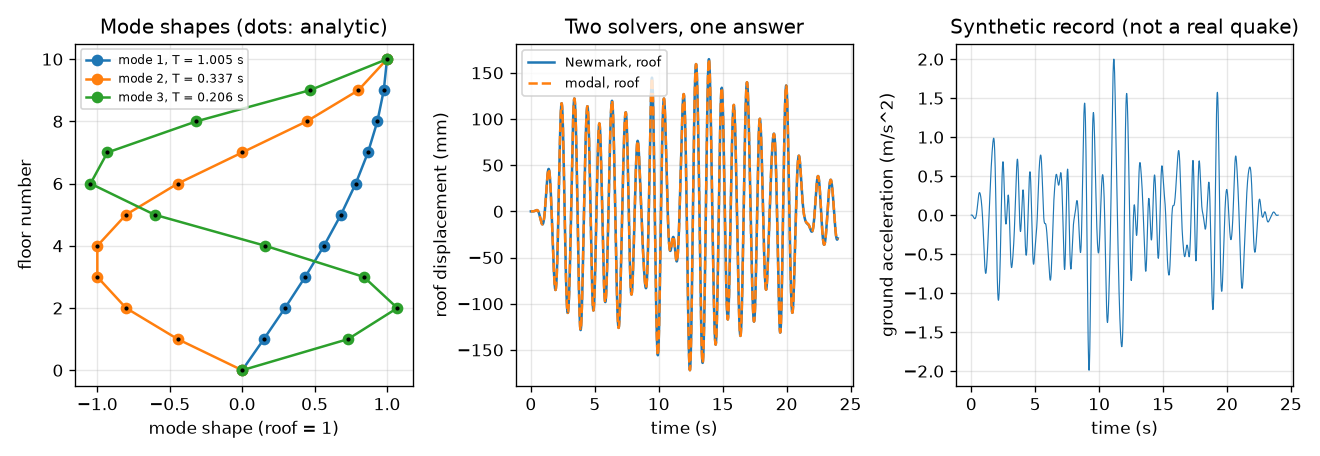
\includegraphics[width=0.85\linewidth]{figures/s03_modes_and_response.png}\\\small Left: first three mode shapes (dots: exact formula). Middle: roof sway from Newmark and from modal superposition. Right: the synthetic ground record.\end{center}

\subsection*{E. Worked example}
Find the periods, mode shapes and effective masses of a two-storey building by hand with m = 200 000 kg and k = 3.5e8 N/m, and check them with the code.
\begin{enumerate}[nosep]
\item K = k [[2, -1], [-1, 1]] and M = m I. With lambda = w\textasciicircum{}2 m / k the eigenproblem is [[2 - lambda, -1], [-1, 1 - lambda]] phi = 0.
\item The determinant condition (2 - lambda)(1 - lambda) - 1 = lambda\textasciicircum{}2 - 3 lambda + 1 = 0 gives lambda = (3 -/+ sqrt 5) / 2 = 0.382 and 2.618.
\item k / m = 1750 per s\textasciicircum{}2, so w1\textasciicircum{}2 = 0.382 * 1750 = 668.4 and w1 = 25.854 rad/s (T1 = 0.2430 s); w2\textasciicircum{}2 = 2.618 * 1750 = 4581.6 and w2 = 67.687 rad/s (T2 = 0.0928 s).
\item From the first row, phi2 / phi1 = 2 - lambda: 1.618 for mode 1 (both floors move the same way; this is the golden ratio, the same number as in the Fibonacci example of Atlas S22) and -0.618 for mode 2 (the floors move in opposite directions).
\item Participation for equal masses: Gamma\textasciicircum{}2 / total mass = (phi1 + phi2)\textasciicircum{}2 / (2 (phi1\textasciicircum{}2 + phi2\textasciicircum{}2)). Mode 1: (2.618)\textasciicircum{}2 / (2 * 3.618) = 0.947. Mode 2: (0.382)\textasciicircum{}2 / (2 * 1.382) = 0.0528. They add to 1.
\end{enumerate}
\textbf{Answer.} T1 = 0.2430 s with shape (1, 1.618) carrying 94.7 percent of the mass, and T2 = 0.0928 s with shape (1, -0.618) carrying 5.3 percent; the code reproduces all of it. For the 10-storey frame the same code gives T1 = 1.0049 s, T2 = 0.3375 s and T3 = 0.2056 s; the first mode carries 84.8 percent of the mass, the second 9.1 percent and the third 3.1 percent.

\subsection*{F. Questions}
\begin{enumerate}[nosep]
\item \textbf{Conceptual.} Why does the first mode carry most of the mass in the response, and why does the second mode have a node (a floor that hardly moves)?
\item \textbf{Numerical.} Two storeys with m = 100 000 kg and k = 1e8 N/m: find both frequencies and periods by hand, then say which mode is more dangerous for a ground period of 1 s.
\item \textbf{Graph and simulation interpretation.} In the soft-storey bar chart, which storey carries the largest drift and how much more than in the uniform frame? What does the damage tell an engineer?
\item \textbf{Design and optimisation challenge.} Design: the first storey is weaker than the others by a factor f (between 0.35 and 1). Find the smallest f in steps of 0.1 that keeps the first-storey drift at no more than 1.5 times the largest drift of the other storeys. Justify the trade-off.
\end{enumerate}

\section{Real-world mini-project}
\textbf{Is this 10-storey frame in danger from a 1 s ground period? Fix it by stiffening.} A 10-storey frame has floors of 200 tonnes, storeys of 350 MN/m each, storey height 3.5 m and 5 percent damping. The city's dominant ground period is 1 s. First show that the frame is in danger: compute its first period and the amplification factor T1 / Tg from Session 2. Then use \texttt{peaks} from Session 3 to stiffen every storey by a factor from 1.0 to 4.0 in steps of 0.5. A stiffening passes when the peak roof sway is at most half of the original and the peak inter-storey drift ratio (drift divided by 3.5 m) is at most 0.5 percent.

\section{The path ahead}
\begin{enumerate}[nosep]
\item \textbf{Session 4: Response-spectrum shortcut.} A function that takes the response spectrum of the record and the modal data of the 10-storey frame and returns a base-shear estimate.
\item \textbf{Session 5: Rayleigh damping instead of modal damping.} A damping matrix built from two coefficients that give 5 percent at modes 1 and 3.
\item \textbf{Session 6: Tune the mass damper.} A search over damper tuning and damper damping, averaged over six random records.
\item \textbf{Session 7: A real record and real periods.} A loader for a public ground-motion record, with the dominant period found from its Fourier spectrum.
\item \textbf{Session 8: Yielding and torsion.} Elastic-perfectly-plastic storeys in the Newmark solver, and a plan-view model with an eccentric mass.
\end{enumerate}

\section{Answers and hints}

\subsection*{Session 1}
\begin{enumerate}[nosep]
\item \textbf{Conceptual.} Hint: Think of a child on a swing: what changes if the child is heavier? Then think about when a push adds to the motion and when it works against it. Solution: A larger mass is harder to accelerate for the same spring force, so each swing takes longer; a stiffer spring pulls back harder for the same sway, so each swing is quicker. That is T = 2 pi sqrt(m / k). When the ground's period equals the building's, every shove arrives just as the building is already moving the same way, so the effects add up cycle after cycle and only damping limits the sway. Even small pushes can build up to a large sway: at 5 percent damping the gain at resonance is 10.
\item \textbf{Numerical.} Hint: w = sqrt(k / m), then T = 2 pi / w. Check the units: k / m is in N/m per kg = 1/s\textasciicircum{}2. Solution: w = sqrt(20 000 000 / 500 000) = sqrt(40) = 6.325 rad/s. T = 2 pi / 6.325 = 0.9935 s. That is within 1 percent of the 1 s ground period, so this building is almost at resonance and would be strongly amplified (about 10 times). Sanity check: it is heavier than the worked example (200 000 kg, T = 0.628 s), so its period is longer.
\item \textbf{Graph and simulation interpretation.} Hint: The ratio is r = T / Tg = building period over ground period. Use the formula or read the curve. Solution: With Tg = 2 s, r = 0.5 and the gain is 1.33: the building mostly follows the slow ground motion, a little amplified. With Tg = 0.5 s, r = 2 and the gain is 0.33: the shaking is too quick for the building to follow, so it hardly moves. Both are far from the resonance peak of 10 at Tg = 1 s.
\item \textbf{Design and optimisation challenge.} Hint: Invert T = 2 pi sqrt(m / k) to get k = m (2 pi / T)\textasciicircum{}2, then use r = T / Tg in the gain formula. Solution: For T = 0.5 s: k = 200 000 * (2 pi / 0.5)\textasciicircum{}2 = 3.158e7 N/m, r = 0.5, gain 1.33. For T = 1.5 s: k = 200 000 * (2 pi / 1.5)\textasciicircum{}2 = 3.509e6 N/m, r = 1.5, gain 0.79. Both avoid the resonance peak of 10. Downsides: the stiff design costs a lot more column material (9 times the stiffness of the flexible one) and attracts larger forces; the flexible design is cheaper but sways a long way in total (a long period means large displacements) and may be uncomfortable or hit the next building. Assumptions: the ground has one steady period and the model is one lump.
\end{enumerate}

\subsection*{Session 2}
\begin{enumerate}[nosep]
\item \textbf{Conceptual.} Hint: Think of the three cases: pushing very slowly, at the natural rhythm, and very quickly. Solution: For r near 0 the push is so slow that the building just follows it statically (D = 1). Near r = 1 the push is in step with the building's own swing, so energy is added every cycle and only damping limits the growth, giving D about 1 / (2 zeta). For large r the push reverses before the heavy roof can respond, so the roof hardly moves (D \textless{} 1, and D falls as r grows). More damping removes energy faster and lowers the peak: 25, 10, 5 and 2.5 for damping ratios 0.02, 0.05, 0.1 and 0.2; it changes the curve little far from resonance.
\item \textbf{Numerical.} Hint: w = sqrt(k / m); r = T / Tg; u\_max = (a0 / w\textasciicircum{}2) D. Solution: w = sqrt(4e6 / 1e5) = sqrt(40) = 6.325 rad/s; T = 2 pi / 6.325 = 0.9935 s; r = 0.9935; D = 1 / sqrt((1 - 0.987)\textasciicircum{}2 + (0.0994)\textasciicircum{}2) = 9.98; a0 / w\textasciicircum{}2 = 2 / 40 = 0.05 m; u\_max = 0.05 * 9.98 = 0.499 m. Sanity check: r is almost 1, so D is almost 10 and the sway is almost half a metre. Units: a0 / w\textasciicircum{}2 is (m/s\textasciicircum{}2) / (1/s\textasciicircum{}2) = m.
\item \textbf{Graph and simulation interpretation.} Hint: At r = 1 the formula collapses to 1 / (2 zeta). Solution: At r = 1: D = 25, 10, 5 and 2.5, which is 1 / (2 zeta) in each case. Halving the damping doubles the peak. At r = 1.5 and zeta = 0.05, D = 0.794: the building is shaken faster than its own rhythm and moves less than the static push would.
\item \textbf{Design and optimisation challenge.} Hint: Use r = 0.7107 and r = 1.2186 (from D = 2) with T = r Tg, then k = m (2 pi / T)\textasciicircum{}2 and u\_max = (a0 / w\textasciicircum{}2) * 2. Solution: Stiff side: T = 0.7107 * 1.5 = 1.066 s, k = 6.948e6 N/m, sway = 0.115 m. Flexible side: T = 1.2186 * 1.5 = 1.828 s, k = 2.363e6 N/m, sway = 0.339 m. Both have D = 2, but the flexible building sways nearly three times further (0.339 against 0.115 m) because a0 / w\textasciicircum{}2 grows with the period, even though it needs much less stiffness. The stiff design keeps displacements small, which protects partitions and neighbours; it costs more column material and attracts larger forces. The flexible one needs a way to cope with large displacement. Assumptions: steady sine ground motion, one lump, 5 percent damping.
\end{enumerate}

\subsection*{Session 3}
\begin{enumerate}[nosep]
\item \textbf{Conceptual.} Hint: Look at the mode shapes: in which mode do all floors move the same way? Then look at the effective masses. Solution: In mode 1 all floors move in the same direction, so the ground pushes all of them in step: the participation Gamma = phi\textasciicircum{}T M r is largest, and 84.8 percent of the mass (10 storeys) takes part. In mode 2 the top moves against the middle: pushes on the two groups of floors partly cancel and only 9.1 percent takes part. Mode 2 changes sign once along the height, so one floor sits near a node. Higher modes have more sign changes and less mass. That is why a handful of modes (here three, 97 percent) is enough.
\item \textbf{Numerical.} Hint: w\textasciicircum{}2 = lambda k / m with lambda = (3 -/+ sqrt 5) / 2, so k / m = 1000 per s\textasciicircum{}2. Solution: w1\textasciicircum{}2 = 0.382 * 1000 = 381.97 so w1 = 19.544 rad/s and T1 = 0.3215 s; w2\textasciicircum{}2 = 2.618 * 1000 = 2618.0 so w2 = 51.167 rad/s and T2 = 0.1228 s. Both periods are far shorter than 1 s, so the ratio T / Tg is below 0.33 for both and neither is near resonance; mode 1 (0.3215 s) is the closer one. Units: k / m is 1/s\textasciicircum{}2, w is in rad/s.
\item \textbf{Graph and simulation interpretation.} Hint: Compare the two bars in storey 1 and also look at the rest of the storeys. Solution: Storey 1: 95.3 mm with a soft first storey against 25.1 mm in the uniform frame, 3.8 times as much, as drift ratio 2.7 percent against 0.72 percent. The other storeys stay near their normal drift. The weak storey concentrates the bending: the whole building above it moves with it, so the first-storey columns take the damage. This is the typical failure of buildings with an open ground floor.
\item \textbf{Design and optimisation challenge.} Hint: Use \texttt{soft\_storey\_stiffness(factor=f)}, run Newmark and compare the first drift with the maximum of the others. Solution: At f = 0.6 the first-storey drift is 55.4 mm, 1.71 times the largest other drift: fails. At f = 0.7 it is 43.5 mm, 1.46 times: passes. So f = 0.7 (the first storey at least 70 percent as stiff as the others) is the smallest with margin; f = 0.35 gives 2.97 times. Trade-off: stiffening the ground floor costs structure and may attract more force; f = 1 gives 1.01 times, a uniform drift. Assumptions: this one synthetic record, linear behaviour, uniform masses.
\end{enumerate}

\section{How to join}
Read \texttt{CONTRIBUTING.md} in the repository, then pick an issue labelled \texttt{good first issue}. Repository: \url{https://github.com/KrunalPanchal1995/openbuildingsway}

\end{document}
